\section{Technical Approach}
To infer information about Java code we use existing Java inference tools and 
combine their output. Additionally we have our own framework which allows us to
implement our own analysis. 

To combine all analysis tools (including our own ones) we have to bring 
their results into a common format at some point in our toolchain. 
We will use the JAIF (Java Annotation Index File) format as our common format. 
Firstly because the Javarifier tool generates its output in this file format. 
Secondly because there do exist tools which allow to extract annotations from 
annotated byte code. This makes it easy to use existing tools which embed their 
results into the byte code.

\begin{figure}
\centering
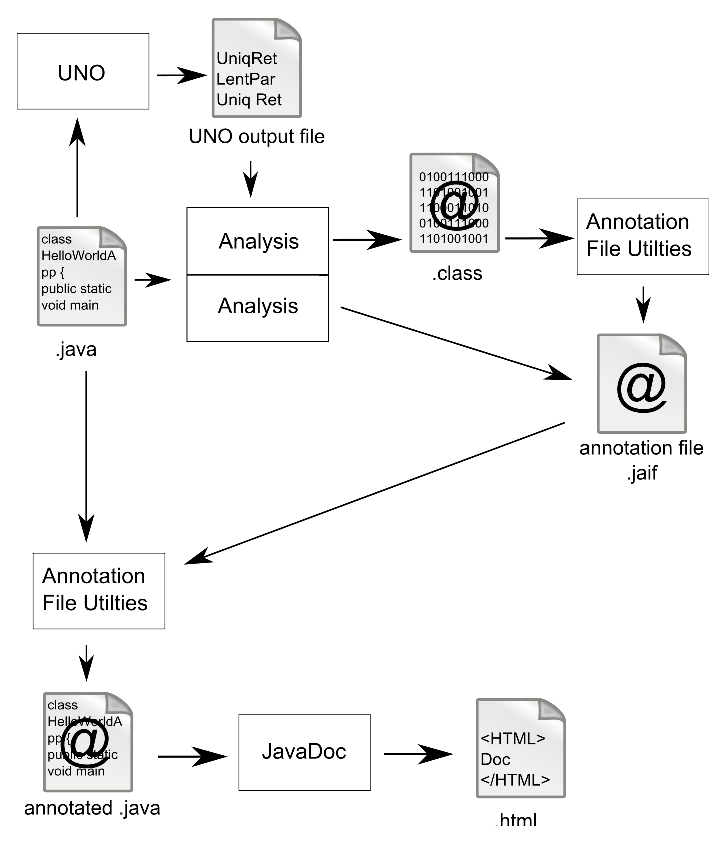
\psfig{file=figures/technicalApproach/technicalApproach.eps, width=3in}
\caption{Toolchain}
\label{fig:toolchain}
\end{figure}

In the following section we describe how our own analysis is built up.
In the sections~\ref{sec:Javarifier} until~\ref{sec:Nullability} we show how each analysis 
generates information and transforms it's result to the JAIF format. In the section~\ref{sec:jaif2html}
we explain how we will use all the annotated files to generate a documentation summarizing
the findings of all the analysis techniques.

\subsection{Analysis Framework}
\label{ss:analysisFramework}

To implement our own analysis tools we use the current version of the Java 7 compiler.
This allows us to use it's plugin architecture to write our own analyzers. From within
a Java compiler plugin we can access the compiler's abstract syntax tree of the 
compilation unit and we can emit 
annotation to the byte code files. As mentioned above those annotation will get extracted 
with the annotation file utilities.

\subsection{Javarifier}
\label{sec:Javarifier}

Javarifier is a tool to infer reference immutability information built in
conjuction with research done by Quinonez et al.~\cite{Javarifier}. It infers
mutability constraints for object fields, method arguments and receivers. Those
constraints may be \texttt{mutable}, \texttt{readonly}, \texttt{?~readonly},
\texttt{polyread}, and \texttt{this-mutable}. The \texttt{?~readonly}
constraint indicates a method argument with a \texttt{readonly} upper bound and
a \texttt{mutable} lower bound. The \texttt{polyread} constraint provides
polymorphism over mutability for method arguments and receivers
(i.e. indicating that a method is read-only when called through a read-only
reference or mutable when called through a mutable reference). A
\texttt{this-mutable} reference provides similar polymorphism for object
fields: a \texttt{this-mutable} field is mutable if \texttt{this} is mutable
and read-only otherwise.

Javarifier produces its results directly in the JAIF format which allows us to
easily integrate it into our toolchain. We need simply to express the meaning
of its inferred constraints in the Javadoc documentation in concise language.

\subsection{Uno}

Uno is an open source tool which is the outcome of a research work done by
Ma and Foster~\cite{Uno}. It infers alias and encapsulation properties for Java.
The tool generates annotations which provide information about how a certain function
treats it's parameters, return objects and fields (in case of a non-static function) 
when called. E.g. if a function captures or leaks a reference or returns a new 
unique reference.

The tool generates annotations which are stored in a single separate file. We plan
to either change the output mechanism of the tool in a way that it directly generates
JAI files or to write a rewriter which transforms files from Uno's file format to the
JAIF format.

In case we realize that the tool is not fulfilling our needs we will implement
our own (simpler) analysis based on the uniqueness inference algorithm
described in~\cite{UniquenessInference}.

\subsection{Thrown Exceptions}

A common frustration with under-documented libraries is that although checked
exceptions might provide information about some of the exceptions thrown, it is
often undocumented what causes certain exceptions to be thrown.  A method that
throws an \texttt{IllegalArgumentException} but has no documentation about what
the expected range for various arguments might be is not helpful.  Buse and
Weimer already infer documentation for what conditions cause some
exceptions~\cite{autodoc}.  Their analysis locates explicit throws of exceptions
and performs some symbolic execution along with propagating results between
methods to determine exceptional input conditions.  Our inference of exceptional
conditions is modeled after
theirs, but we will implement our own inference because we can find no existing
implementation of such an analysis that is readily available.

\subsection{Nullability}
\label{sec:Nullability}
In heavily object oriented languages like java, every variable is a nullable (aka. option, maybe) type, capable of holding either a reference to a value or the special value null.  Because of this ubiquity, one common mistake is to call methods with null parameters they are unprepared to handle, or to erroneously assume that returned values are never null.  Well documented libraries, like the Java collections framework, will frequently spell out when variables are assumed to be nullable or not-null when an ambiguity seems likely.  By means of a nullability inference\cite{NIT,NonNullTypeInference} we can add similarly useful type decorations (in the form of icons) to documentation.  Although two Java nullability inferences are freely available, they are both whole program analyses and therefore ill-suited to our target application: library documentation.  We plan to first try adapting their existing analysis code, or failing that re-implement a modular version of their analysis within our own framework.

\subsection{From JAIF to HTML documentation}
\label{sec:jaif2html}

To get the inferred information back into the source files we use the annotation 
file utilities (\cite{AFU} AFU). The next step is to run JavaDoc over our
annotated source code. We will need to write a JavaDoc plugin (called doclet) which will
cause JavaDoc to generate documentation for our new annotations. The output will
generate a HTML documentation of the code enriched with automatically inferred
properties expressed in a programmer friendly format.

Figure \ref{fig:toolchain} shows the stages in our toolchain.
